\begin{figure}[htbp]
    \centering
    \begin{subfigure}{0.32\textwidth}
        \centering
        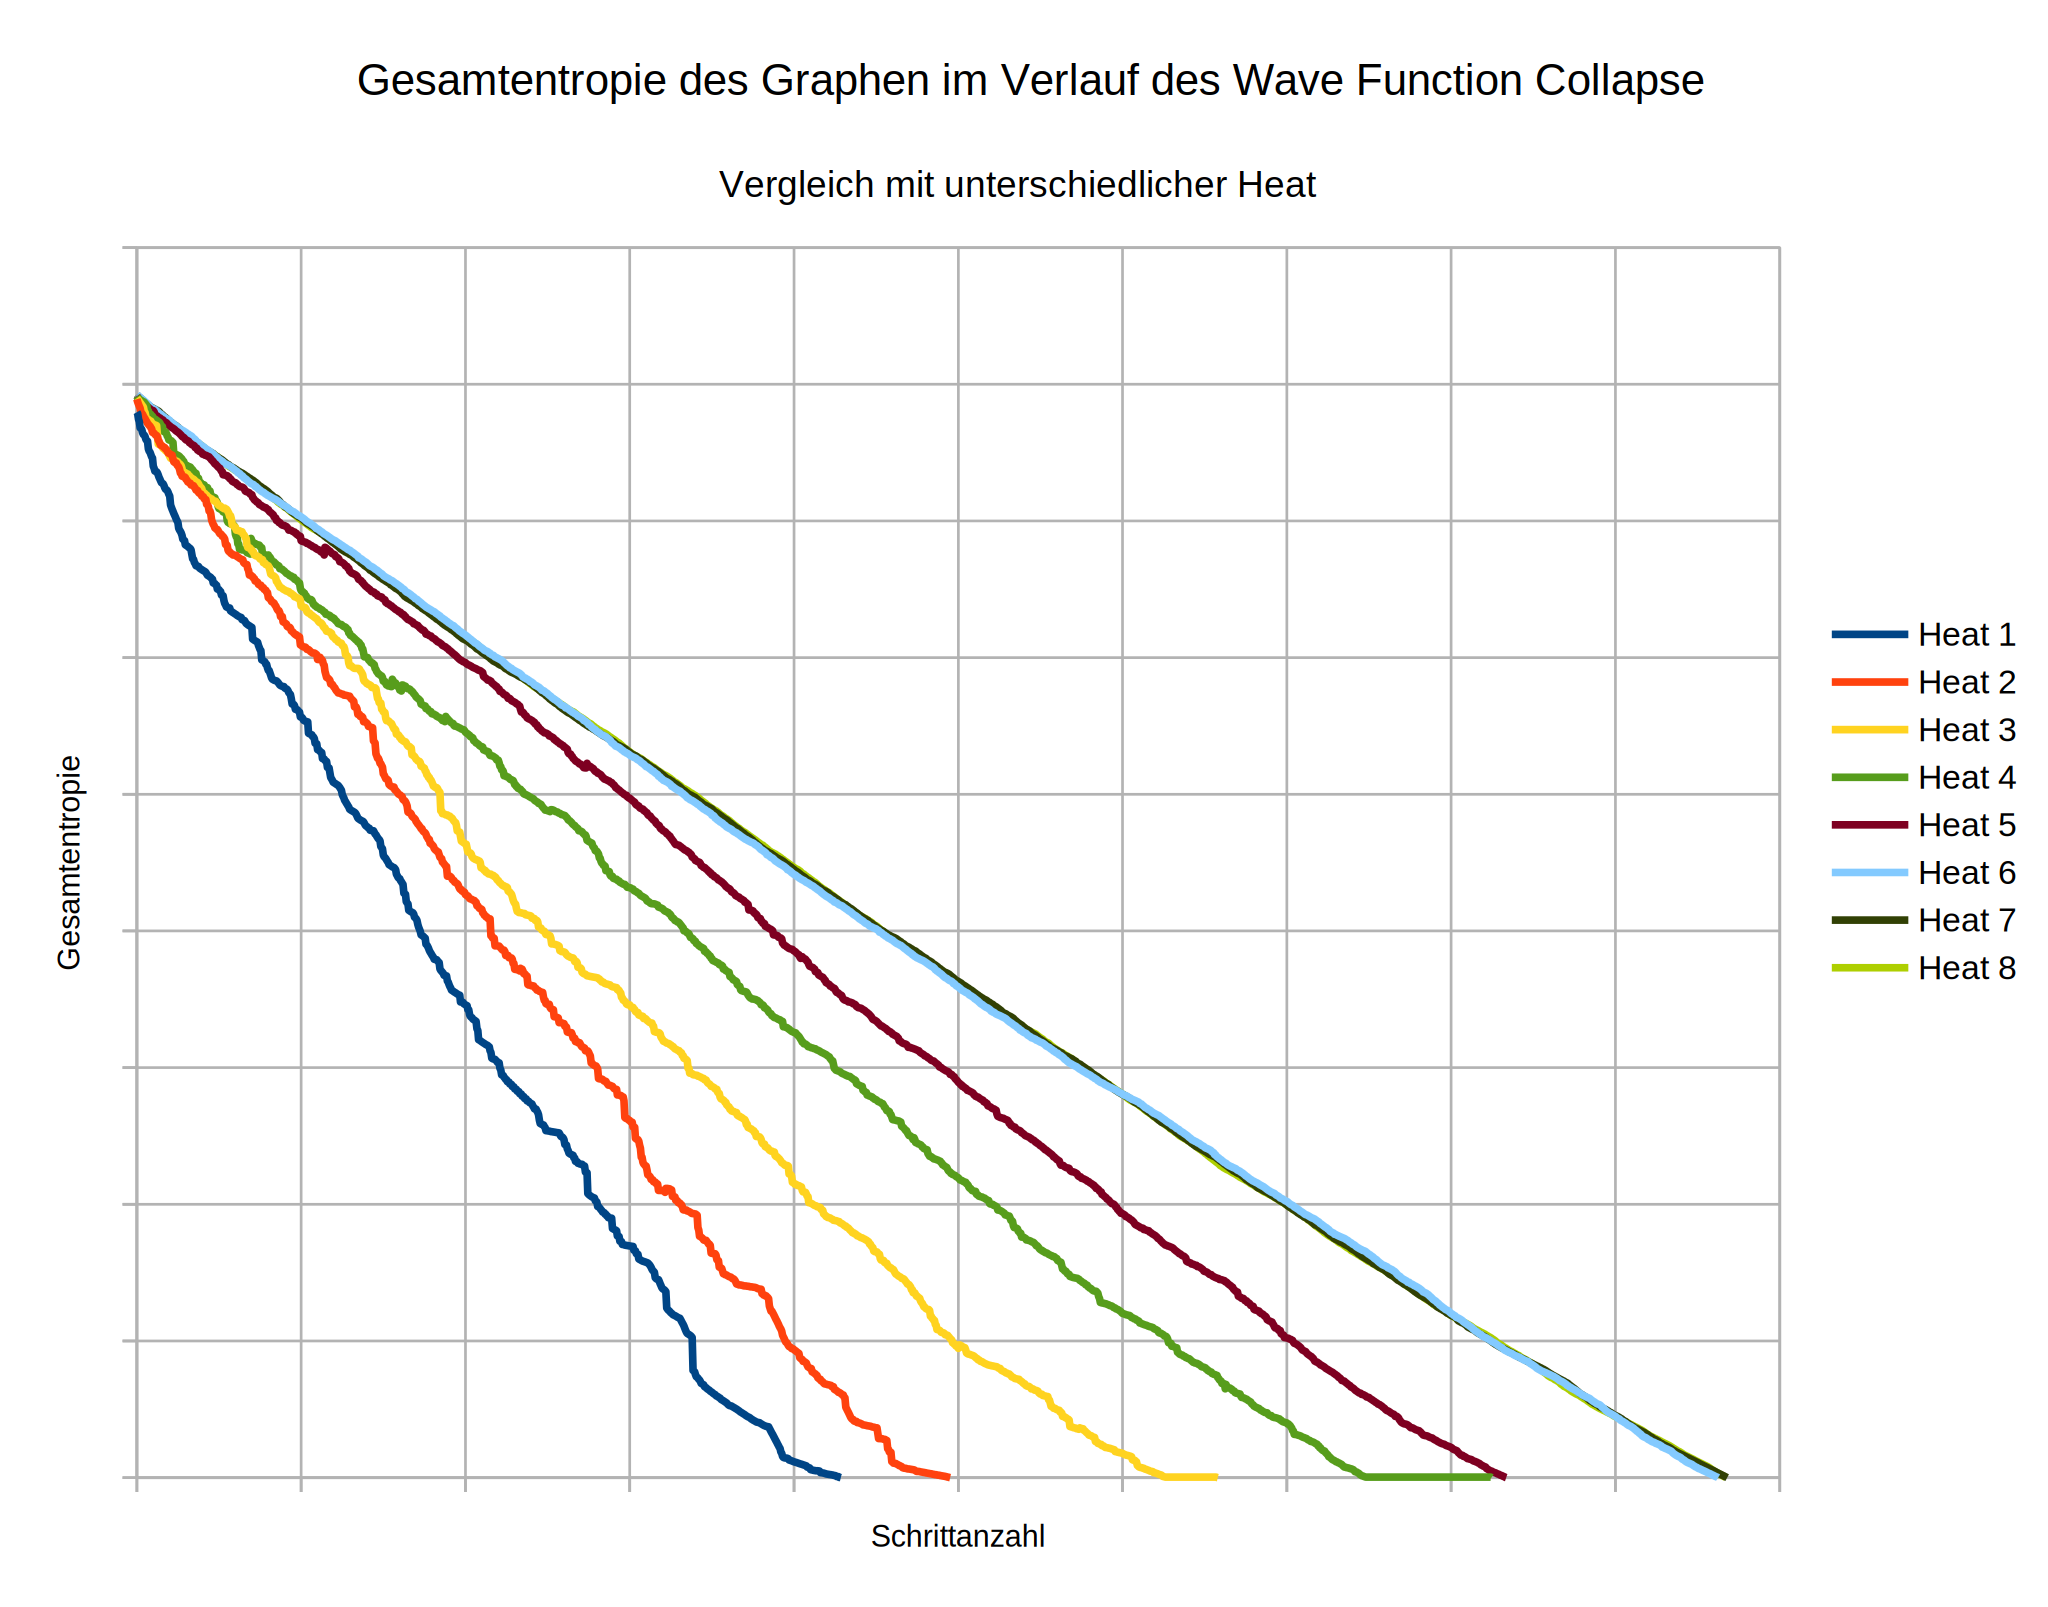
\includegraphics[width=\linewidth]{data/hex_heat/1.png}
        \caption{Quadrate mit Heat=1}
    \end{subfigure}\hfill
    \begin{subfigure}{0.32\textwidth}
        \centering
        \includegraphics[width=\linewidth]{data/hex_heat/2.png}
        \caption{Sechsecke mit Heat=1}
    \end{subfigure}
    \begin{subfigure}{0.32\textwidth}
        \centering
        \includegraphics[width=\linewidth]{data/hex_heat/3.png}
        \caption{Sechsecke mit Heat=2}
    \end{subfigure}\hfill
    \caption{
        Einfluss von Heat auf die Qualität der Ausgabe
    }
    \label{fig:hex_heat}
\end{figure}